\fancyhf{}
\renewcommand{\headrulewidth}{0pt}
\newgeometry{bottom=0.5cm,top=1cm,right=1cm,left=1cm}

\begin{landscape}


\section{Appendix 3 - Class UML Diagrams}
\label{Appendix_3}
\subsection{Booking and Facilities}
\begin{figure}[H]
    \centering
    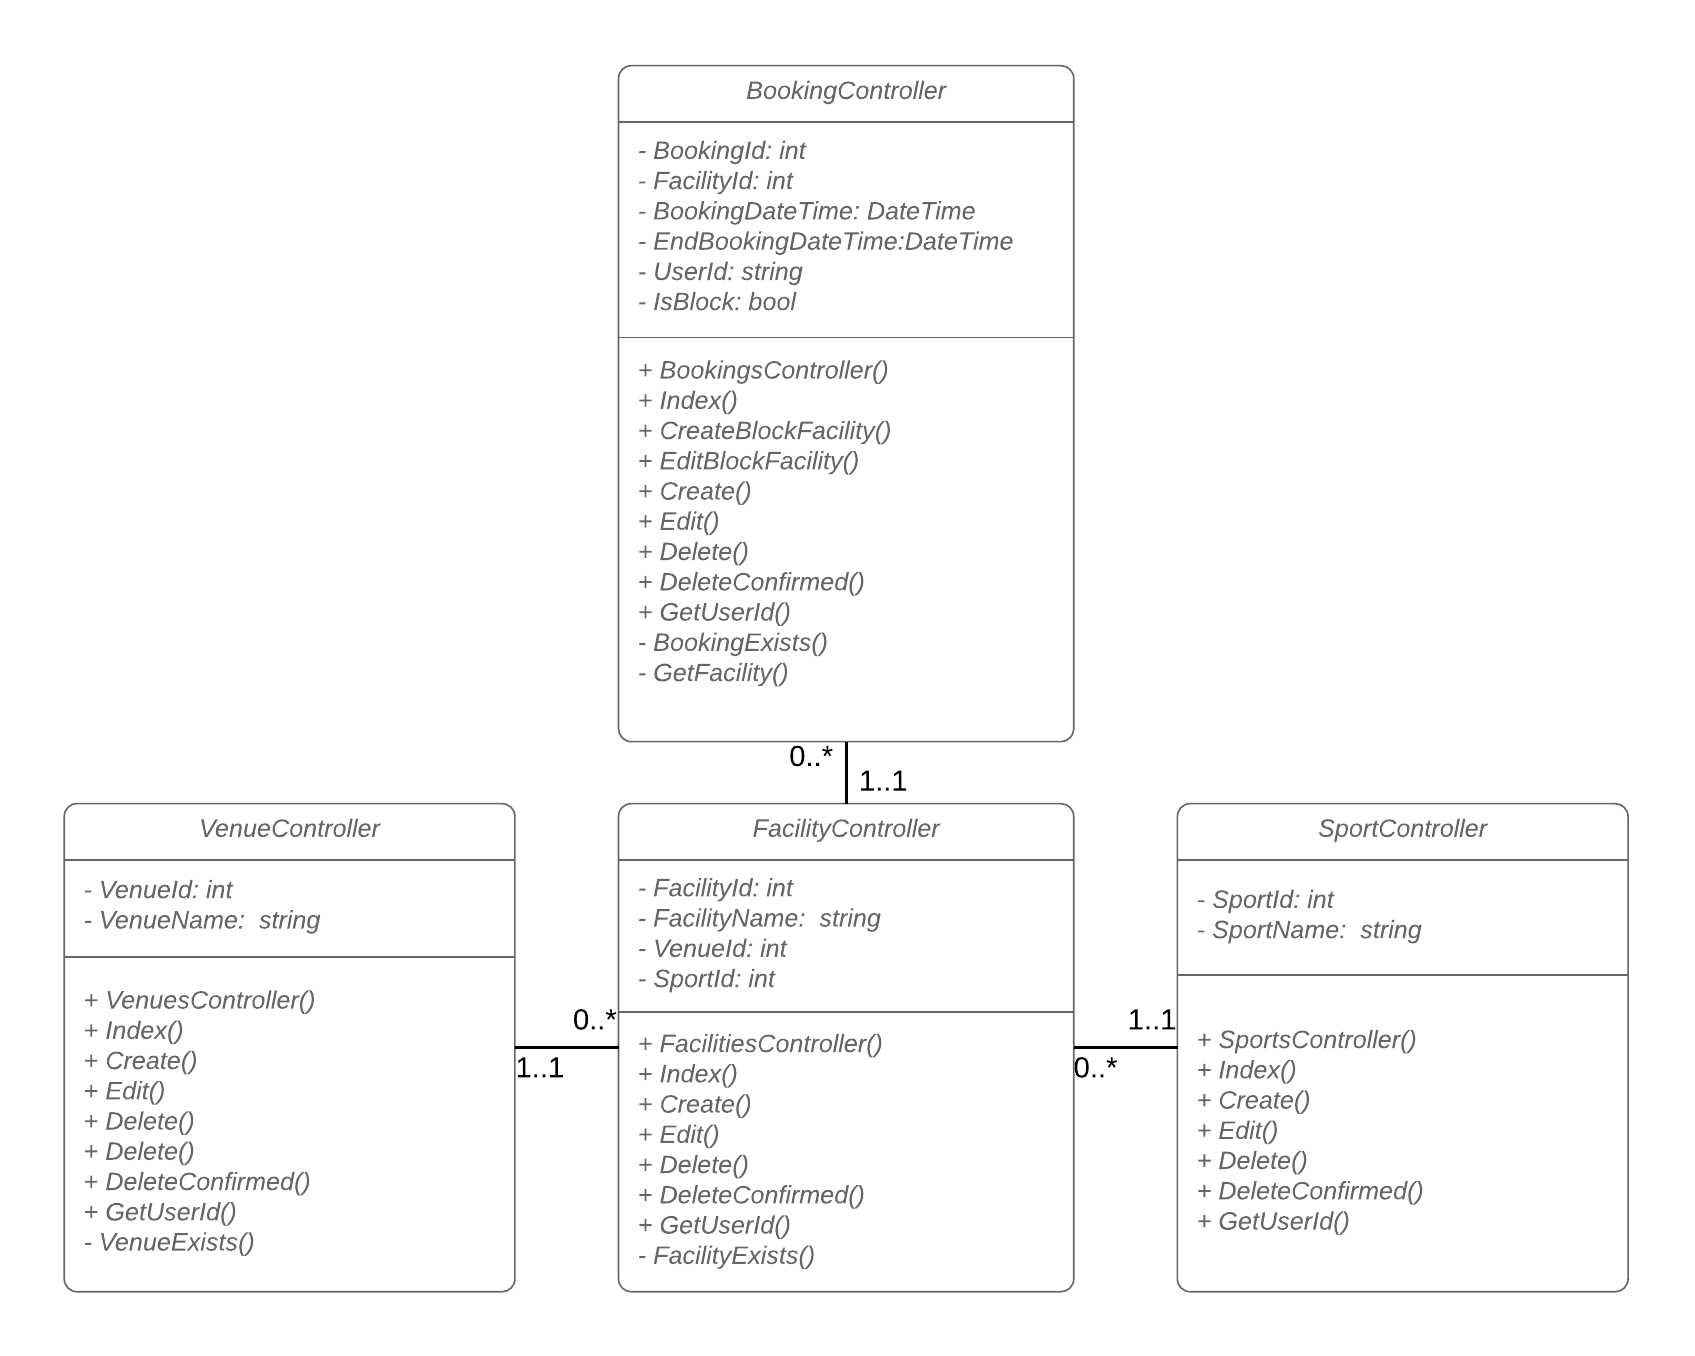
\includegraphics[width=\textwidth]{Images/class_uml/booking_facilities.png}
    \caption{UML Diagram of Classes within the \textit{Booking and Facilities} microservice}
    \label{fig:class_uml:booking-facilities}
\end{figure}
\subsection{Challenges}
\begin{figure}[H]
    \centering
    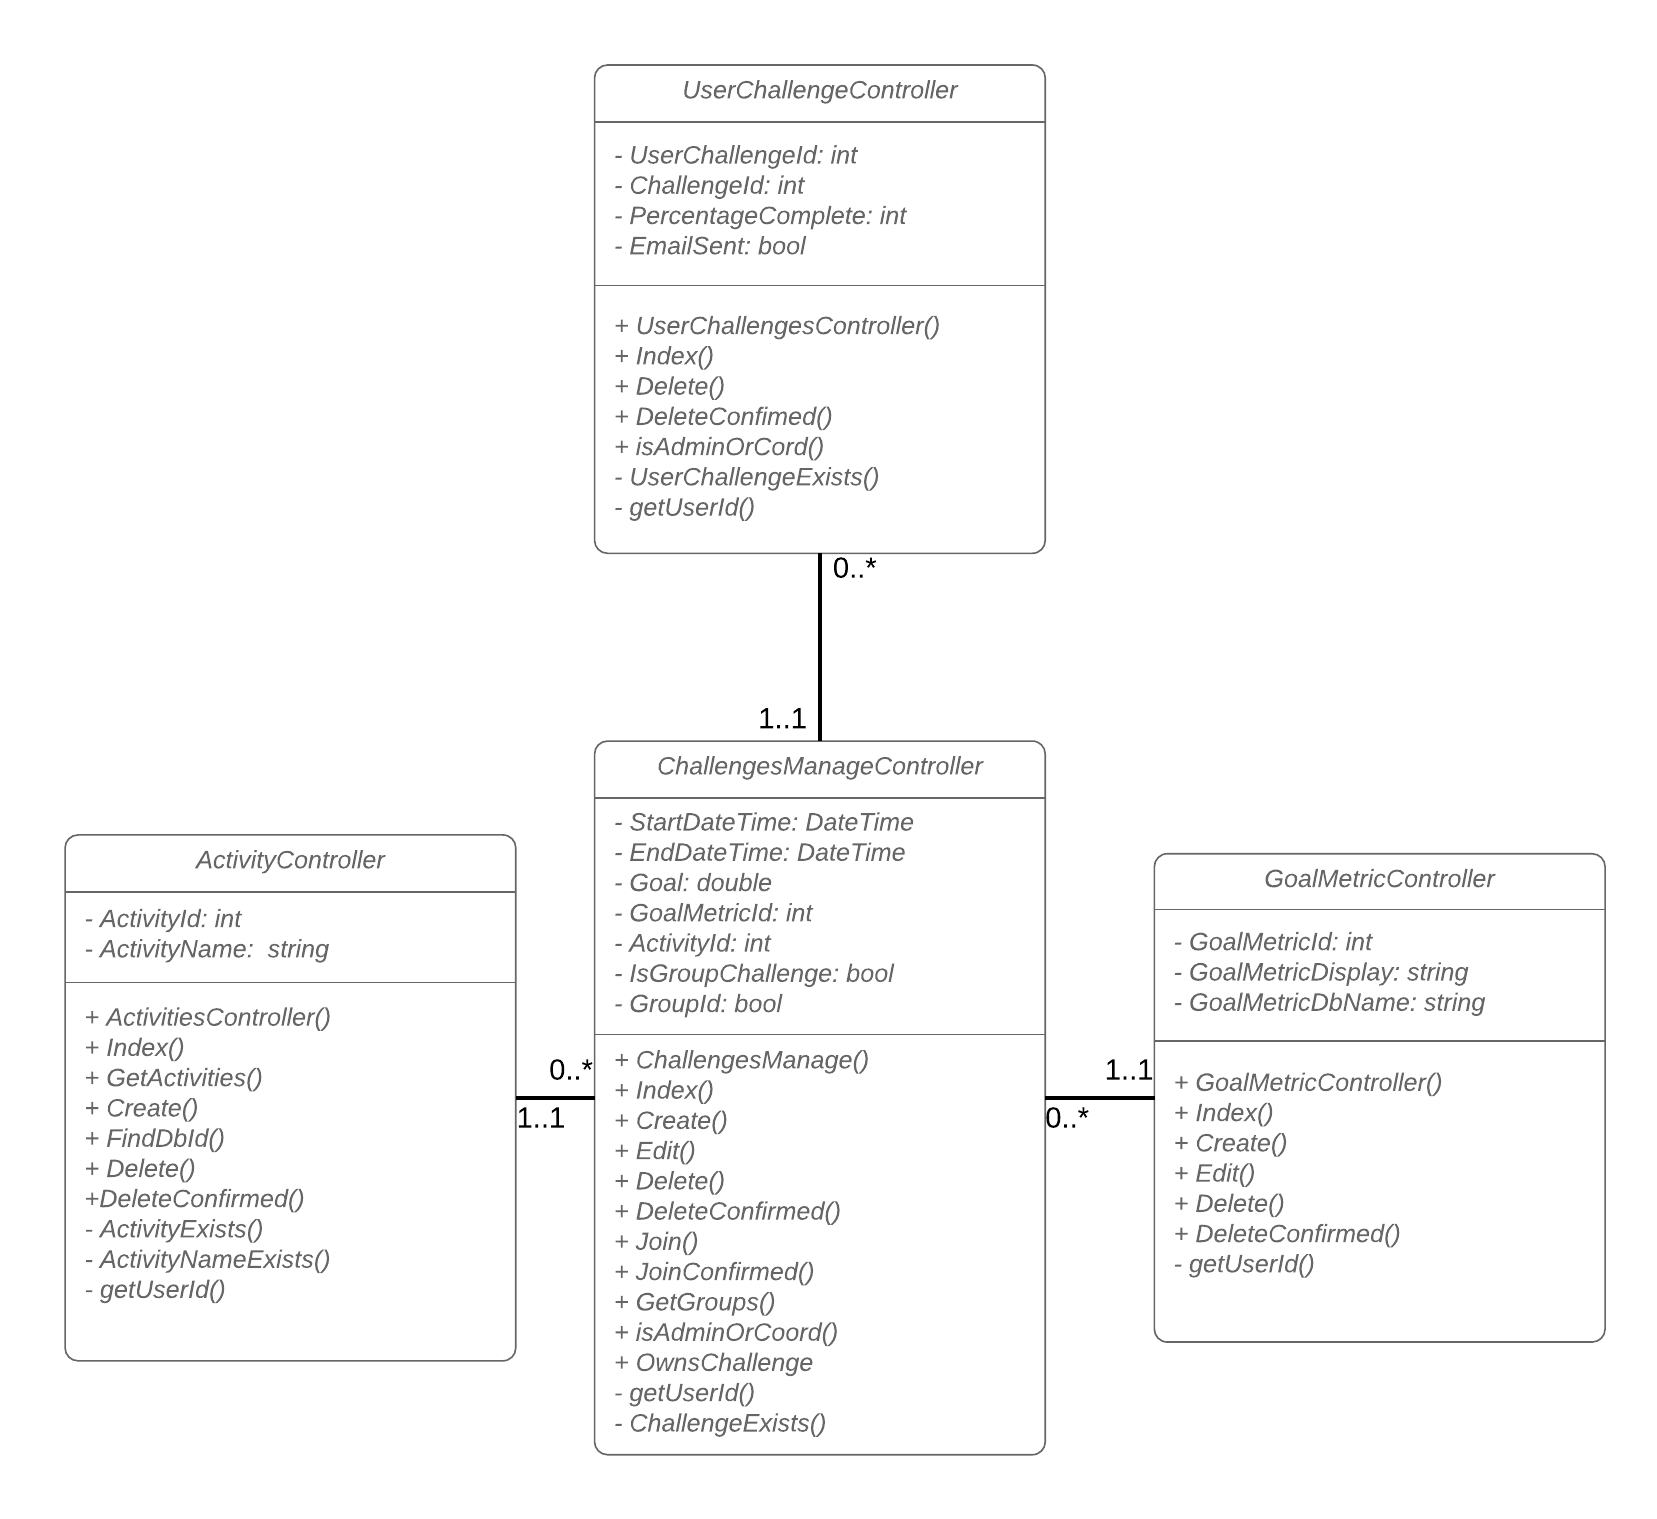
\includegraphics[width=\textwidth]{Images/class_uml/challenges.png}
    \caption{UML Diagram of Classes within the \textit{Challenges} microservice}
    \label{fig:class_uml:challenges}
\end{figure}
\end{landscape}
\subsection{Fitbit Ingest Service}
\label{fig:class_uml:fitbit-ingest-service}
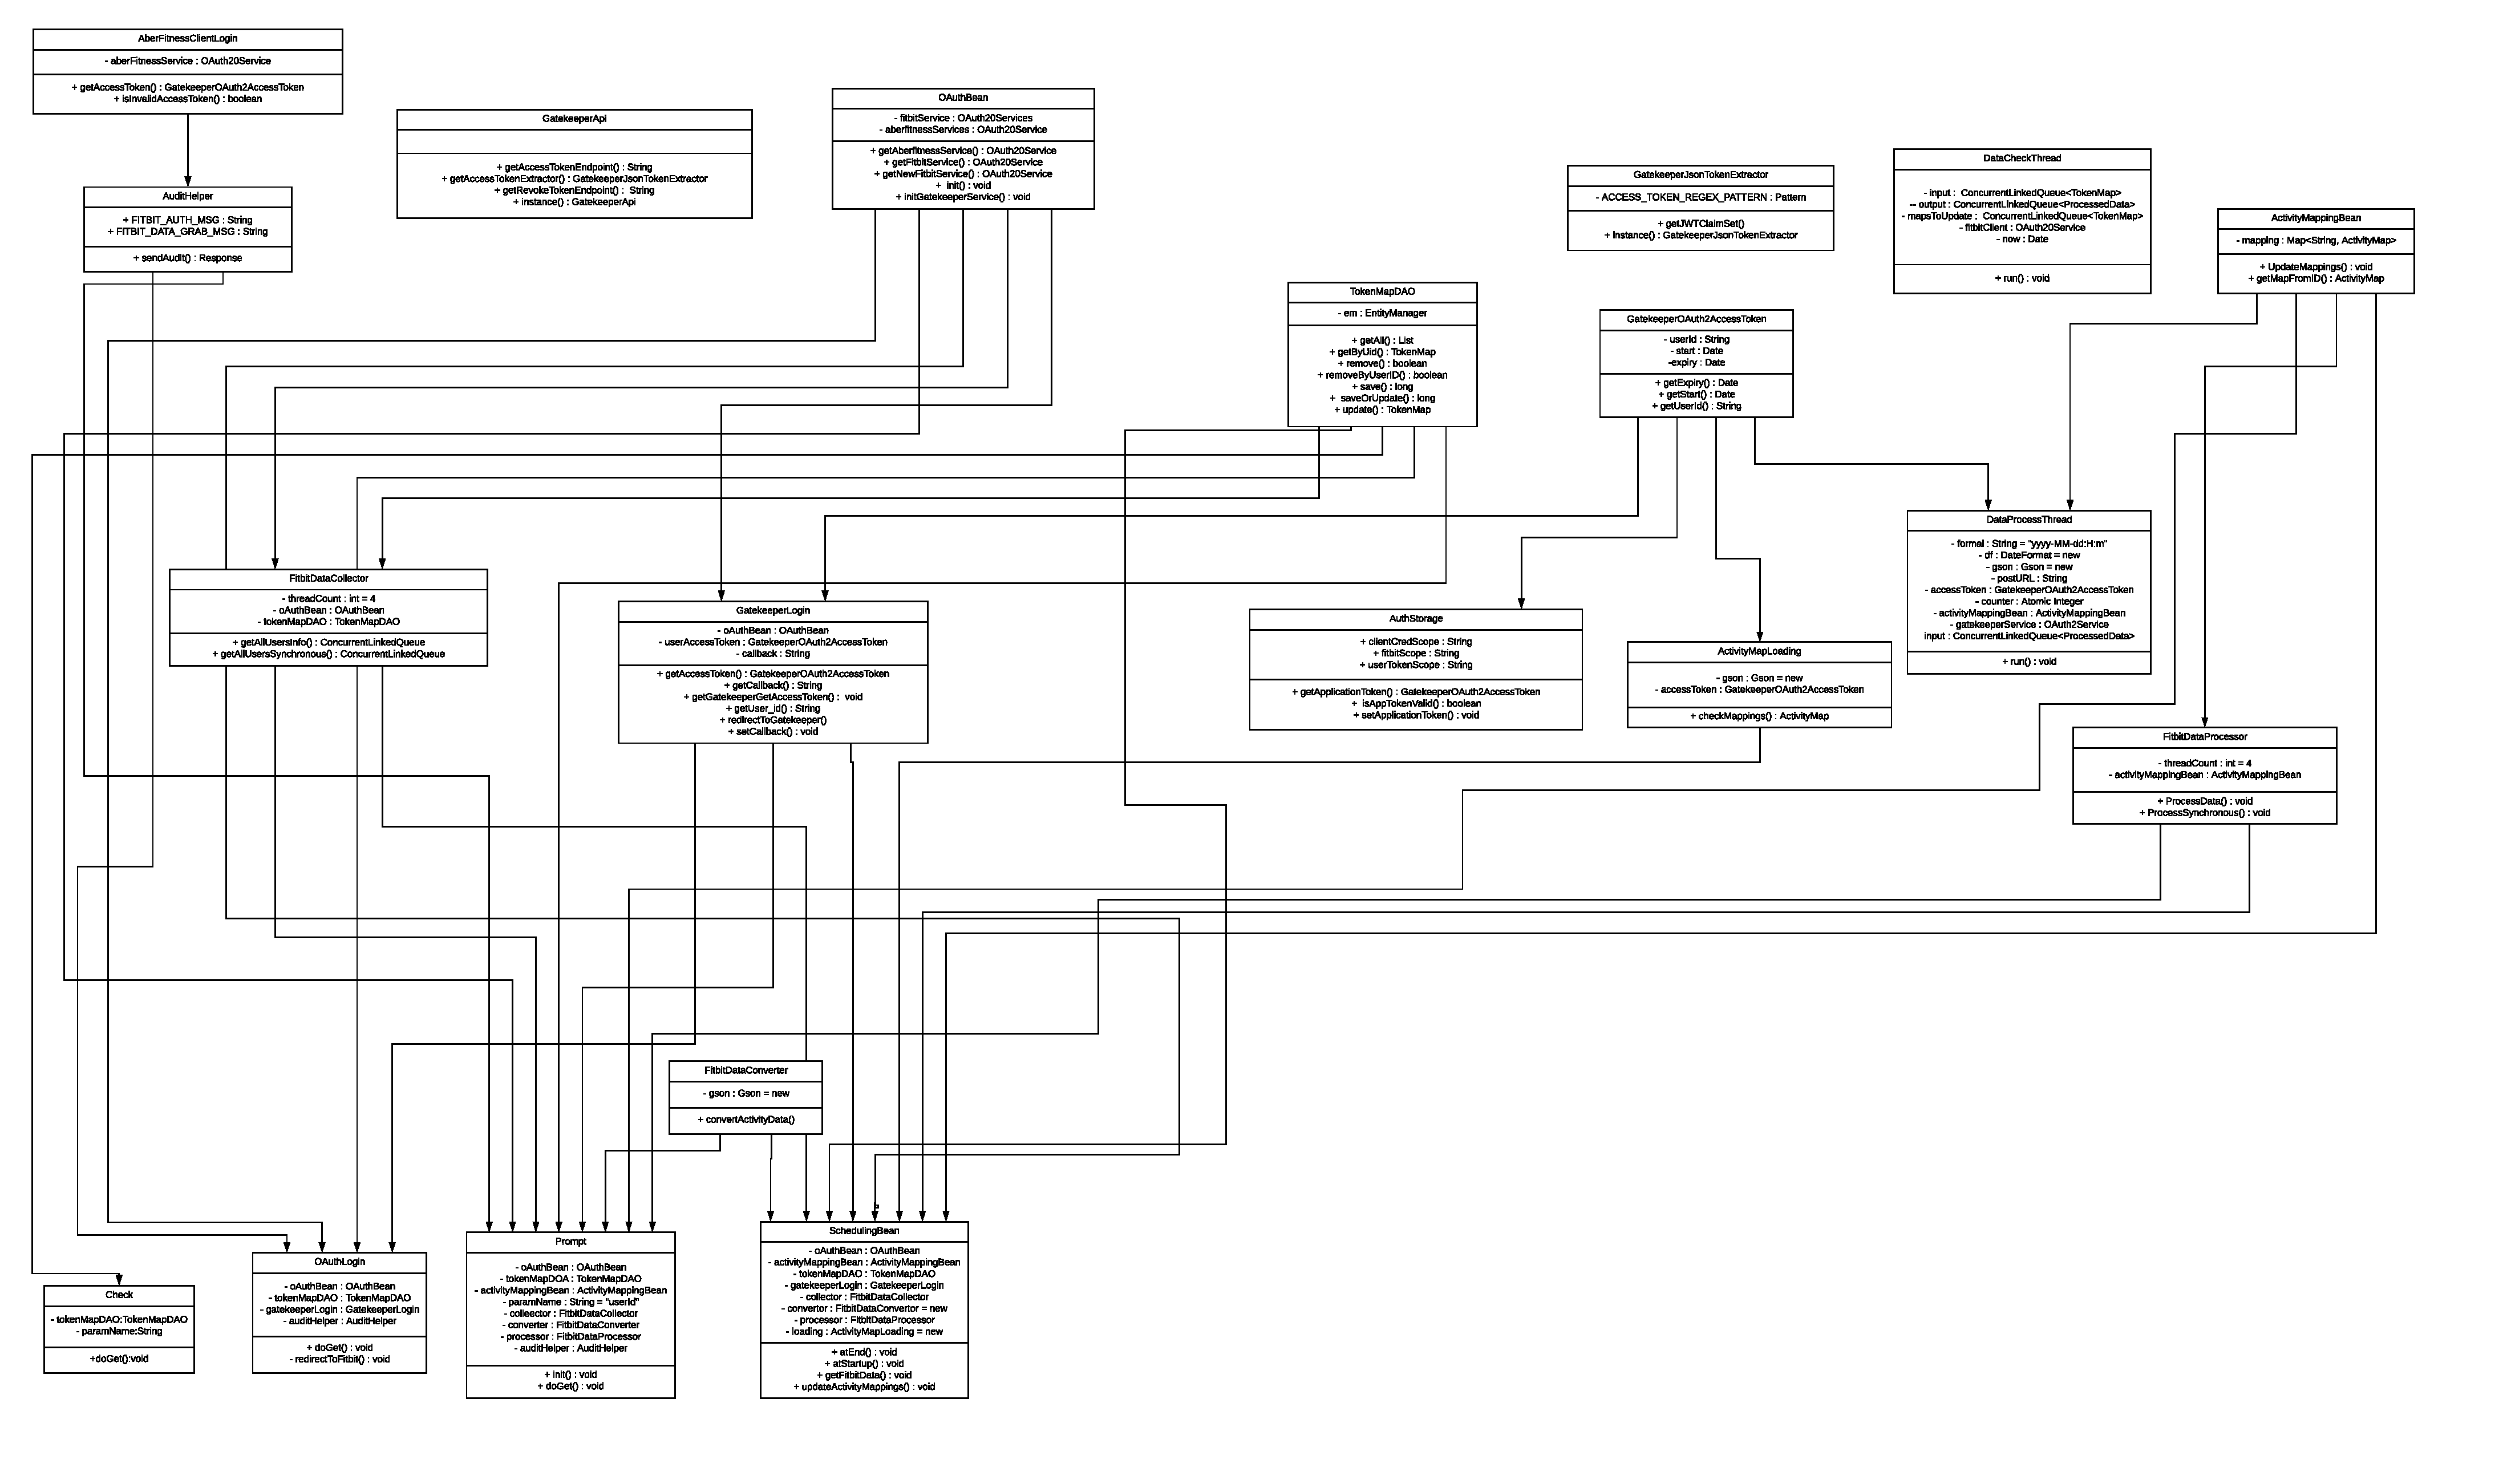
\includepdf[landscape=true]{Images/class_uml/fitbit-ingest-service.pdf}
\subsection{GLaDOS}
\label{fig:class_uml:glados}
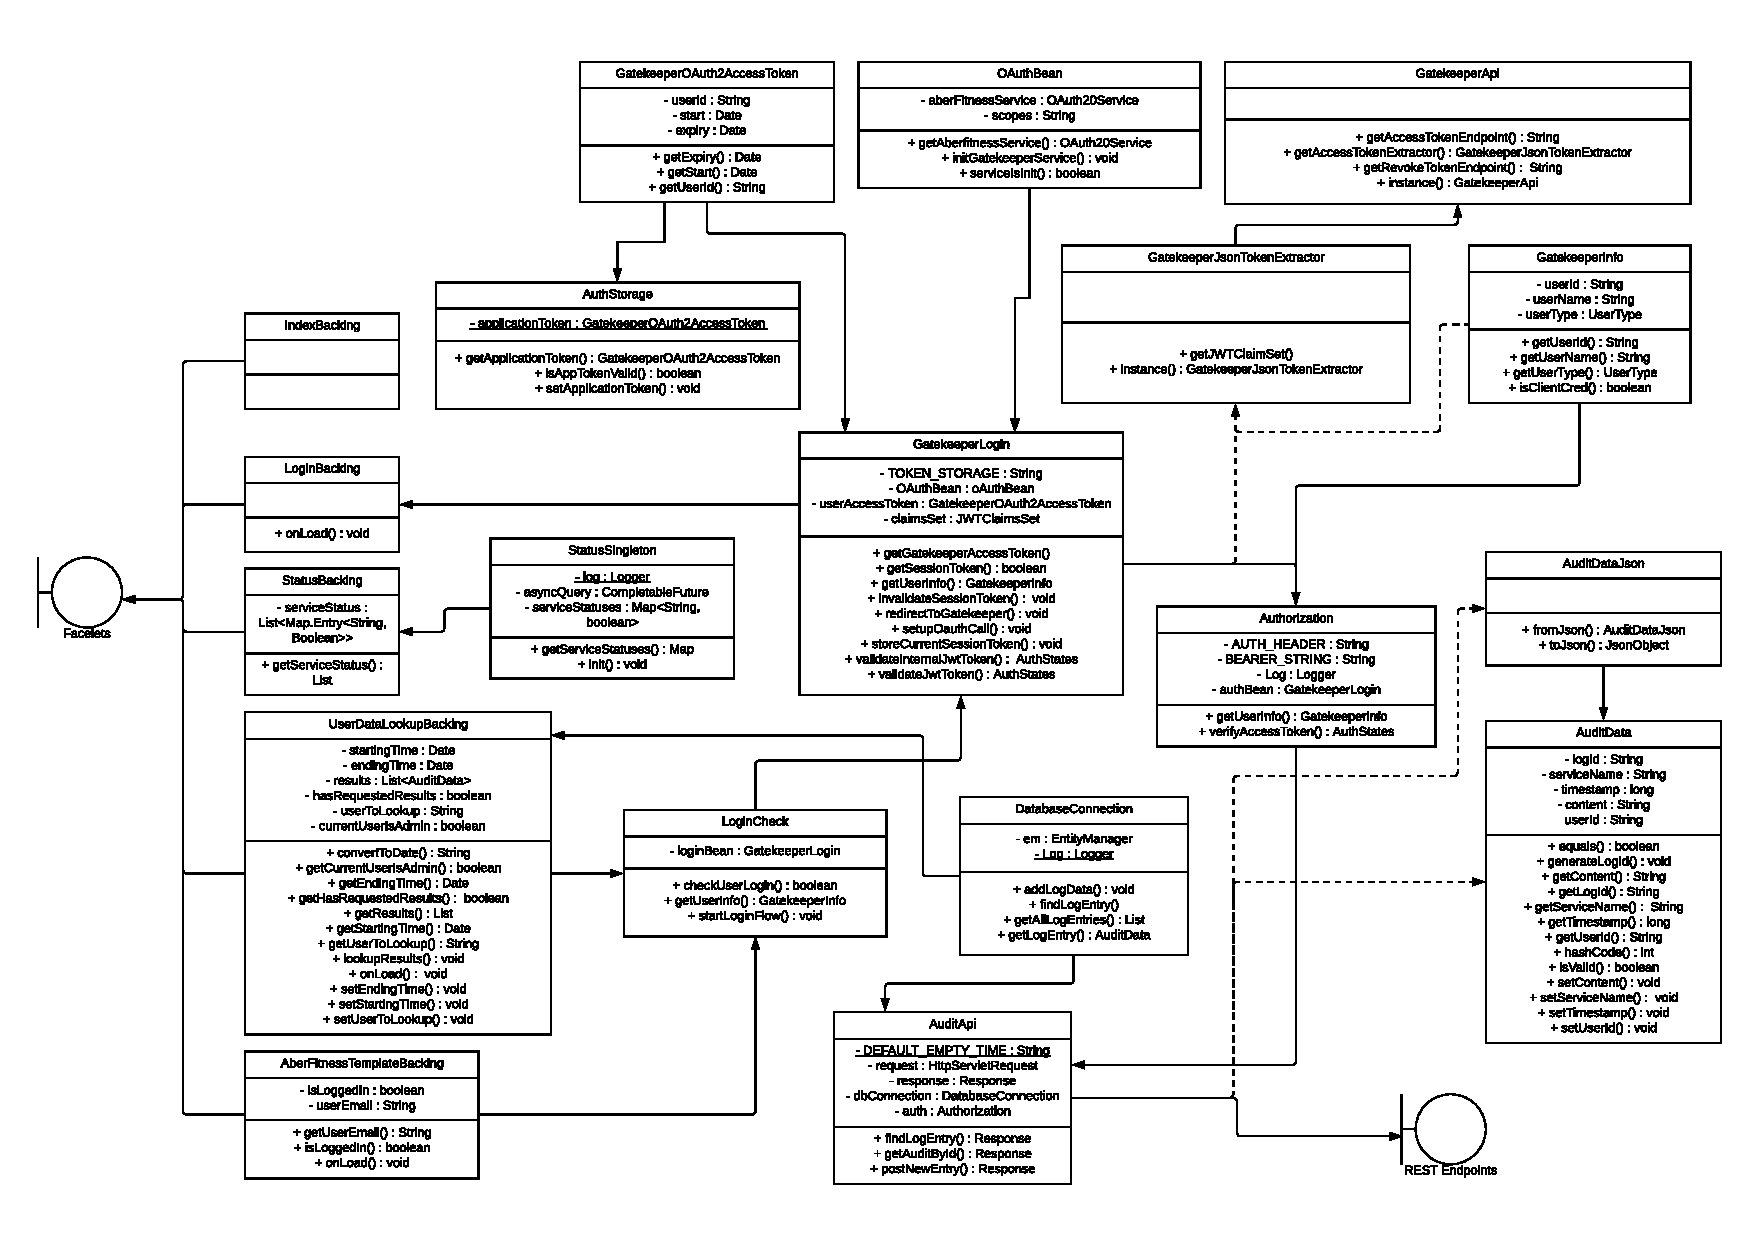
\includepdf[landscape=true]{Images/class_uml/glados.pdf}
\subsection{Ladders}
\label{fig:class_uml:ladders}
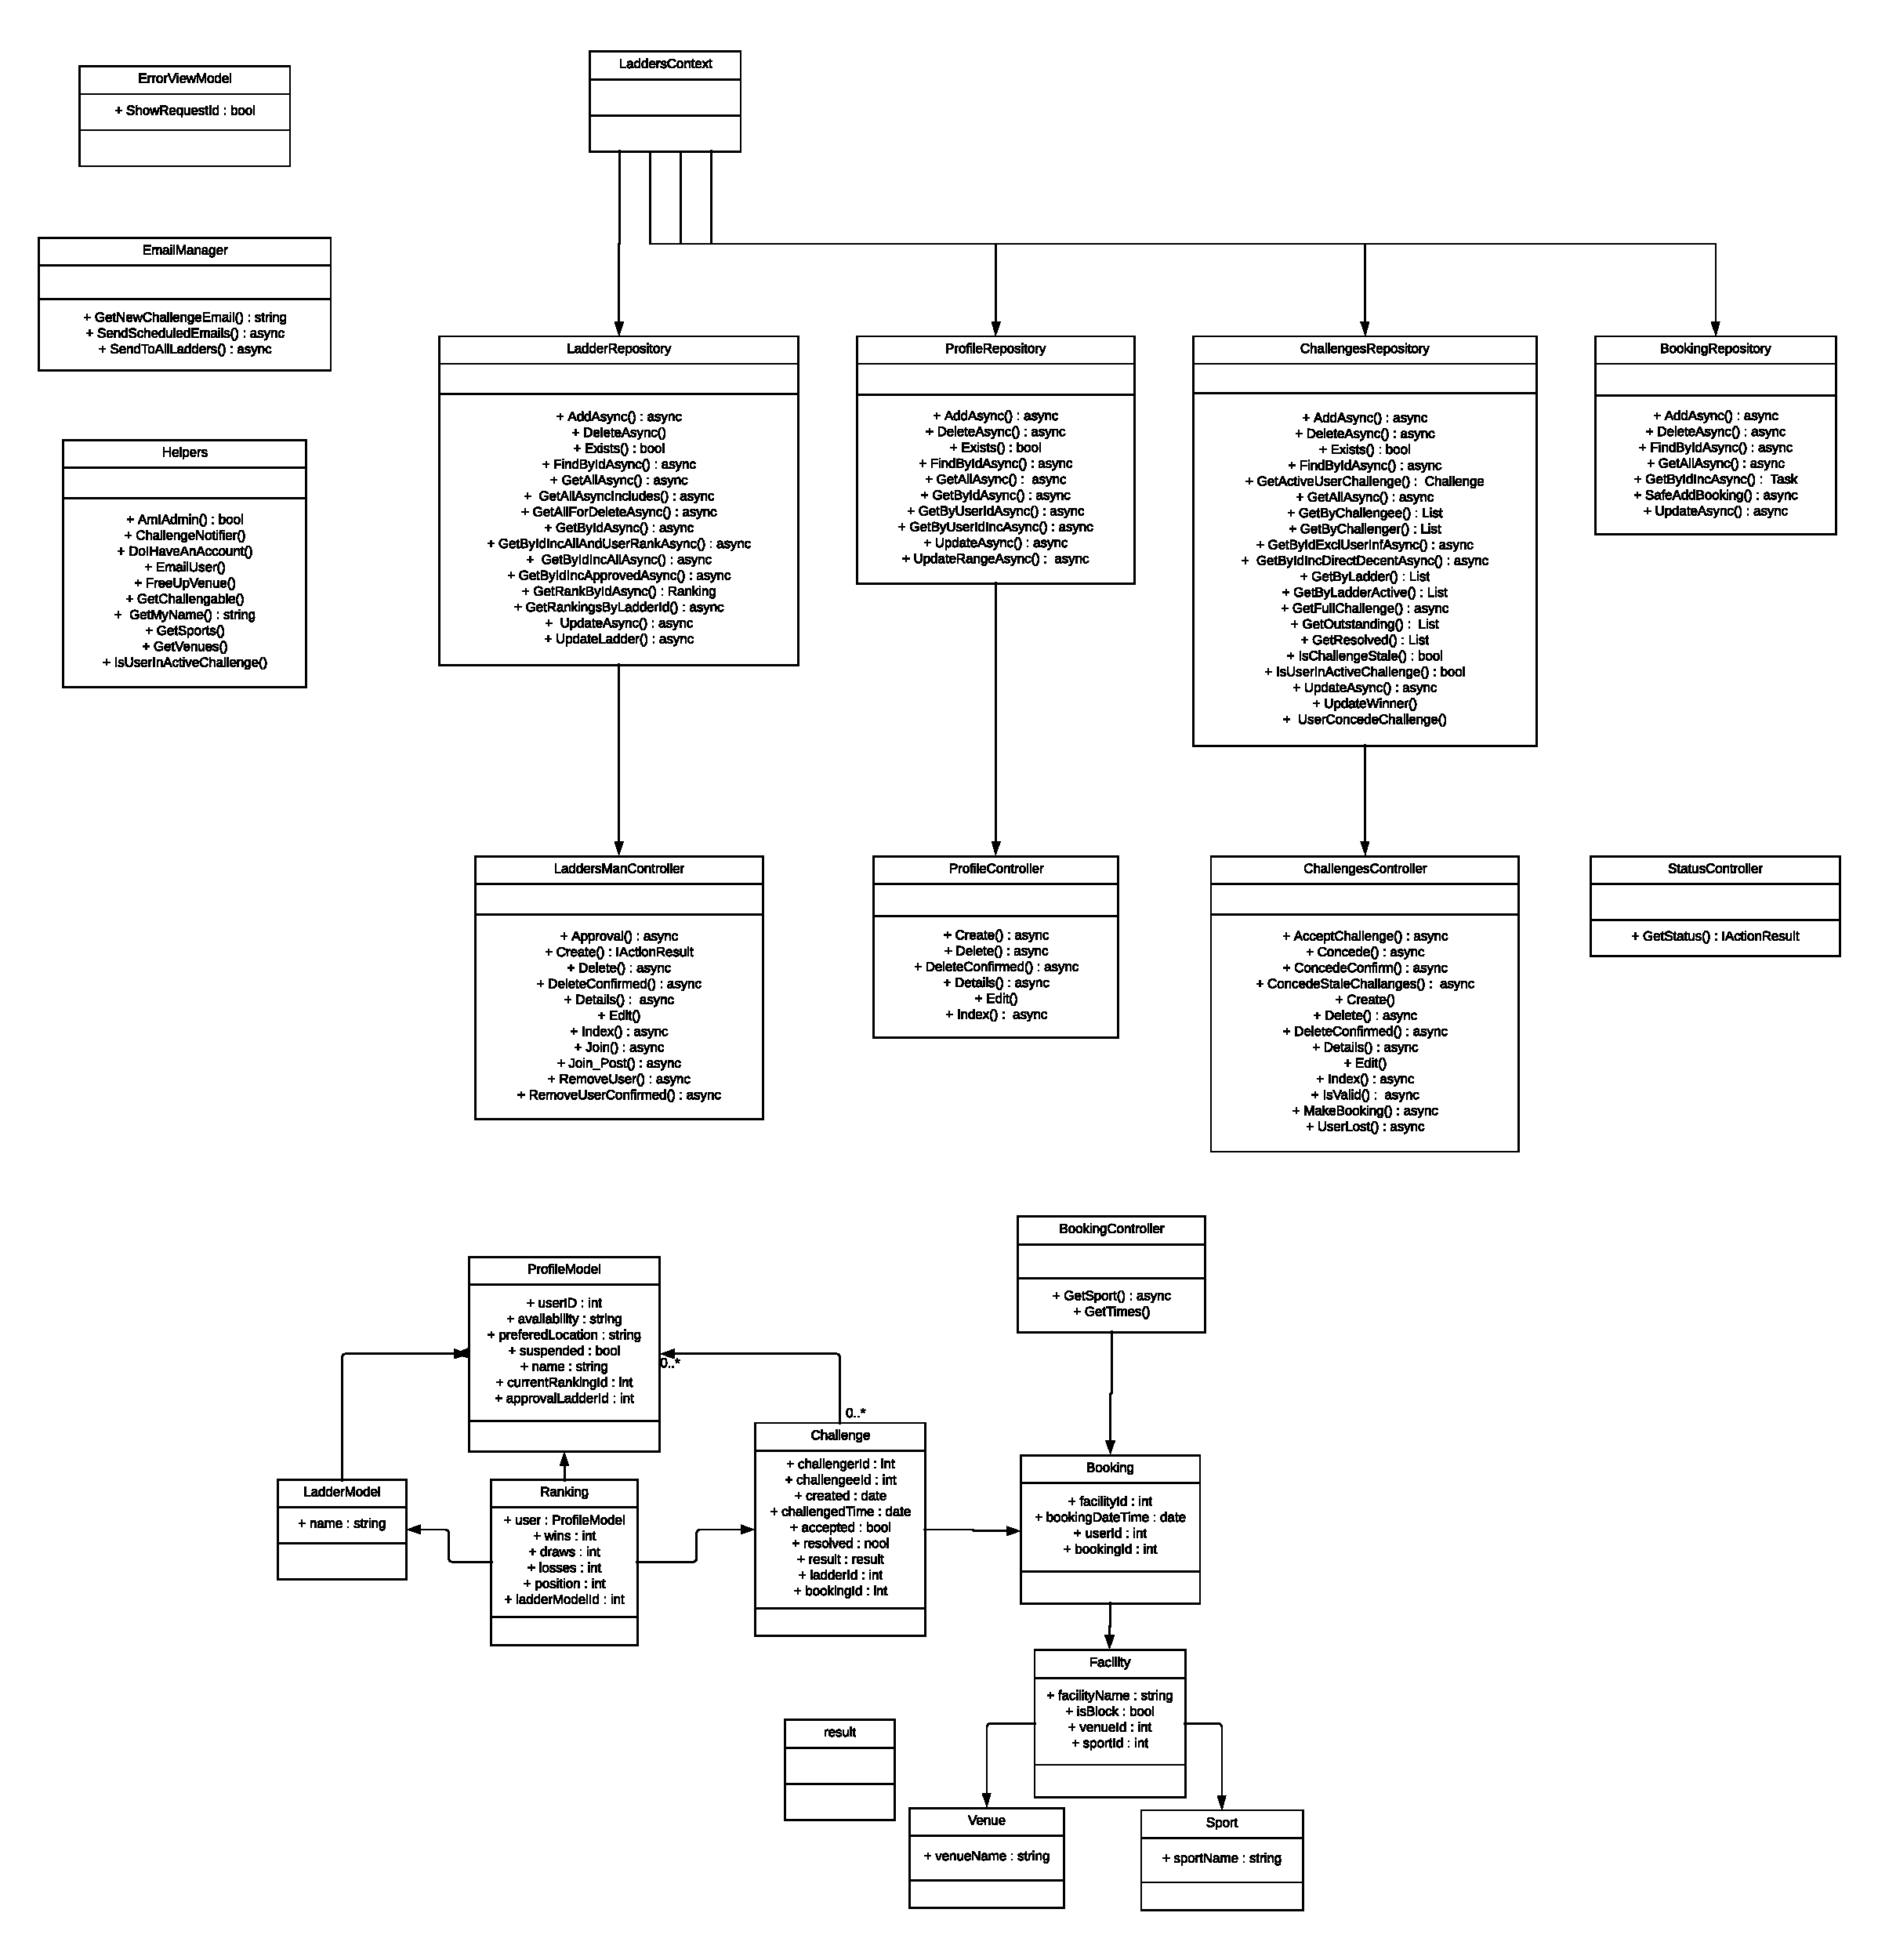
\includepdf[landscape=true]{Images/class_uml/ladders.pdf}



% Reset page styling
\newgeometry{left=10.6mm,right=10.6mm}
\setchapterheaderfooter{} 
\renewcommand{\headrulewidth}{0.4pt}
